\documentclass[11pt, oneside]{article} 
\usepackage{geometry}
\geometry{letterpaper} 
\usepackage{graphicx}
	
\usepackage{amssymb}
\usepackage{amsmath}
\usepackage{parskip}
\usepackage{color}
\usepackage{hyperref}

\graphicspath{{/Users/telliott_admin/Tex/png/}}
% \begin{center} 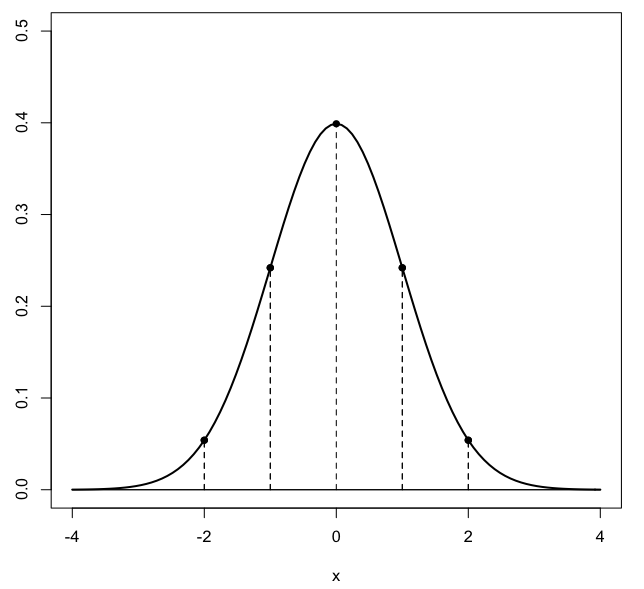
\includegraphics [scale=0.4] {gauss3.png} \end{center}

%break
\title{Orthonormal basis}
\date{}

\begin{document}
\maketitle
\Large

We know that if we start with a matrix with independent columns, we have a "basis" for the space.  That is, we can express any vector as a combination of the columns of $A$.
\[
A=
\begin{bmatrix} 
  3  &  2  &  4 \\ 
  2  &  0  &  2 \\
  4  &  2  &  3
\end{bmatrix} \ \ 
\]
Here, we calculate $det(A) = -(2)(6-8) - (2)(6-8) = 8 \ne 0$.  So we know the columns of $A$ are independent.

However, we are asked to find an orthonormal basis, one with vectors that are orthogonal ("ortho") and unit length ("normal").

One thing to notice before we start:  the sum of the diagonal (called the trace) is $6$, so when we get the eigenvalues they should add up to $6$, while they multiply to give the determinant.
\[
det(A- \lambda I) = 
\begin{vmatrix} 
  3 - \lambda  &  2  &  4 \\ 
  2  &  - \lambda  &  2 \\
  4  &  2  &  3 - \lambda
\end{vmatrix} \ \ 
\]
I will put the three terms of the determinant on separate lines
\[ (3-\lambda)[(-\lambda)(3-\lambda) - 4)] = (3-\lambda)(\lambda^2 - 3\lambda - 4) =  -\lambda^3 + 6\lambda^2 - 5\lambda - 12 \]
\[ (-2)[(2)(3-\lambda) - 8] = (-2)(6 - 2\lambda - 8) = 4\lambda + 4\]
\[ (4)[4 - (4)(-\lambda)] = (4)(4 + 4 \lambda) = 16 + 16 \lambda \]
Adding them all up
\[ - \lambda^3 + 6 \lambda^2 + 15 \lambda + 8 = 0\]
I'm not too good at factoring cubics, but I notice that $\lambda = -1$ is a solution, so that means that $(\lambda + 1)$ is a factor leading to
\[ (\lambda + 1)(-\lambda^2 + 7\lambda + 8) = (-1)(\lambda + 1)(\lambda-8)(\lambda + 1) = 0 \]
So finally we have eigenvalues $\lambda = 8, -1, -1$.  Notice that these do indeed add up to give the trace, and multiply to give the determinant.

Sidestep finding eigenvectors for now

\[ \mathbf{u} = \  \langle 0,-2,1 \rangle  \]
\[ \mathbf{v} = \  \langle 1,-2,0 \rangle  \]
\[ \mathbf{w} = \  \langle 2,1,2 \rangle   \]
$\mathbf{w}$ is the eigenvector for eigenvalue $\lambda = 8$.
Notice that although $\mathbf{u} \perp \mathbf{w}$ and $\mathbf{v} \perp \mathbf{w}$, $\mathbf{u} \cdot \mathbf{v} \ne 0$.  

I didn't mention this before, but notice now that $A$ is a symmetric matrix.  It turns out that the eigenvectors of a symmetric matrix are guaranteed to be orthogonal, \emph{unless there are repeated eigenvalues}.  In that case the combinations of the eigenvectors form what is called an eigenspace, and any vector in that eigenspace will be orthogonal to $\mathbf{w}$.  

This is easily checked.  For constants $c$ and $d$, we have the combinations $c\mathbf{u}$ and $d\mathbf{v}$ are
\[  \langle 0,-2c,c \rangle  +  \langle d,-2d,0 \rangle  \ = \  \langle d,-2c-2d,c \rangle  \]
\[  \langle d,-2c-2d,c \rangle  \cdot  \langle 2,1,2 \rangle  \ = 2d - 2c - 2d + 2c = 0\]

Let's take $\mathbf{w}$ and $\mathbf{v}$ as already orthogonal, and then produce from $\mathbf{u}$ a new vector orthogonal to both.  The formula we want (see the Projections write-up) is
\[ \mathbf{u'} = \mathbf{u} - \frac{w^Tu}{w^Tw}w - \frac{v^Tu}{v^Tv}v \]
\[ \mathbf{w} \cdot \mathbf{u} = 0 \]
So this means that the whole second term is zero.
\[ \mathbf{v} \cdot \mathbf{u} = 4 \]
\[ \mathbf{v} \cdot \mathbf{v} = 5 \]
So we have
\[ \mathbf{u'} = \mathbf{u} - (4/5) \mathbf{v} \]
\[ \mathbf{u} =  \langle 0,-2,1 \rangle  \ = \ (1/5)  \langle 0,-10,5 \rangle  \]
\[ (4/5)\mathbf{v} = (1/5) \  \langle 4,-8,0 \rangle   \]
\[ \mathbf{u'} = \mathbf{u} - (4/5) \mathbf{v} \]
\[ = (1/5)( \langle 0,-10,5 \rangle \ -\  \langle 4,-8,0 \rangle ) \]
\[ = (1/5)  \langle -4,-2,5 \rangle  \]

Check that $\mathbf{u'} \perp \mathbf{v}$ and $\mathbf{u'} \perp \mathbf{w}$.

The last step is to scale these to be unit vectors.  We have 
\[ \mathbf{u'} = (1/5)  \langle -4,-2,5 \rangle  \]
As a unit vector, this is
\[ \mathbf{u'} = (1/3\sqrt{5})  \langle -4,-2,5 \rangle  \]
Then
\[ \mathbf{v} = \  \langle 1,-2,0 \rangle  \]
becomes
\[ \mathbf{v'} = \ (1/\sqrt{5})  \langle 1,-2,0 \rangle  \]
The easiest one is 
\[ \mathbf{w} = \  \langle 2,1,2 \rangle   \]
\[ \mathbf{w'} = \  \langle 2/3,1/3,2/3 \rangle   \]
I want to check that the diagonalization works properly.
\[ \mathbf{u'} = (1/3\sqrt{5})  \langle -4,-2,5 \rangle  \]
\[ \mathbf{v'} = \ (1/\sqrt{5})  \langle 1,-2,0 \rangle  \]
\[ \mathbf{w'} = \ (1/3)  \langle 2,1,2 \rangle   \]
We should have that
\[ Q \Lambda Q^{-1} = A \]
Luckily, for an orthonormal matrix
\[ Q^{-1} = Q^T \]
But even so, I don't want to do this by hand.  In R

\begin{verbatim}
> A = c(3,2,4,2,0,2,4,2,3)
> dim(A) = c(3,3)
> A
     [,1] [,2] [,3]
[1,]    3    2    4
[2,]    2    0    2
[3,]    4    2    3
> result = eigen(A)
> result
$values
[1]  8 -1 -1

$vectors
          [,1]       [,2]       [,3]
[1,] 0.6666667  0.7453560  0.0000000
[2,] 0.3333333 -0.2981424 -0.8944272
[3,] 0.6666667 -0.5962848  0.4472136
\end{verbatim}

Our first vector is $\mathbf{w'}$ (they have listed the largest eigenvalue first).  The second vector is $\mathbf{u'}$.  They have listed the vectors with their components in opposite order (bottom to top).  Remember that $\mathbf{u'}= \langle -4,-2,5 \rangle $ with a factor of $(1/3\sqrt{5}) = 0.1491$, which gives the result shown.

\begin{verbatim}
>>> f = 5**0.5 * 3
>>> 1/f
0.14907119849998599
>>> 2/f
0.29814239699997197
>>> 4/f
0.5962847939999439
>>> 5/f
0.7453559924999299
\end{verbatim}

$\mathbf{v'}= \langle 1,-2,0 \rangle $ with a leading factor of $(1/\sqrt{5}) = 0.4472$.

\begin{verbatim}
>>> f = 5**0.5
>>> 1/f
0.4472135954999579
>>>  2/f
0.8944271909999159
\end{verbatim}

So this also matches.  Now we just do

\begin{verbatim}
> L = diag(result$values)
> L
     [,1] [,2] [,3]
[1,]    8    0    0
[2,]    0   -1    0
[3,]    0    0   -1
> S = result$vectors
> S
          [,1]       [,2]       [,3]
[1,] 0.6666667  0.7453560  0.0000000
[2,] 0.3333333 -0.2981424 -0.8944272
[3,] 0.6666667 -0.5962848  0.4472136
> Si = solve(S)
> Si
          [,1]       [,2]       [,3]
[1,] 0.6666667  0.3333333  0.6666667
[2,] 0.7453560 -0.2981424 -0.5962848
[3,] 0.0000000 -0.8944272  0.4472136
\end{verbatim}

"solve" is R's way of finding the inverse.  Notice that $Q^{-1} = Q^T$, as we said.
\begin{verbatim}
> S %*% L %*% Si
     [,1]         [,2] [,3]
[1,]    3 2.000000e+00    4
[2,]    2 1.776357e-15    2
[3,]    4 2.000000e+00    3
\end{verbatim}

If you round the second column to $ \langle 2,0,1 \rangle $, you will see that we have re-generated A.
\end{document}  